
Charged particles produced in collisions traverse the ID,
depositing on sensors signals that are recorded as spatial coordinates. These
coordinates are then processed through a pattern recognition and
reconstruction algorithm to extract the particle tracks from which the
momentum four vectors are derived (see
section~\ref{chap:reco:sec:tracks}). The ID is designed to measure
tracks across a large momentum range, from $O(100 \mev)$ to $O(1
\tev)$, falling in the pseudorapidity range $|\eta| < 2.5$. It is composed of three
sub-detectors: the pixel tracker, the silicon microstrip tracker
(SCT), and the transition radiation tracker (TRT). A cross-sectional
diagram of the ID in the barrel region is shown in
figure~\ref{chap:detector:fig:inner_detector}.

\begin{figure}[ht]
    \centering
    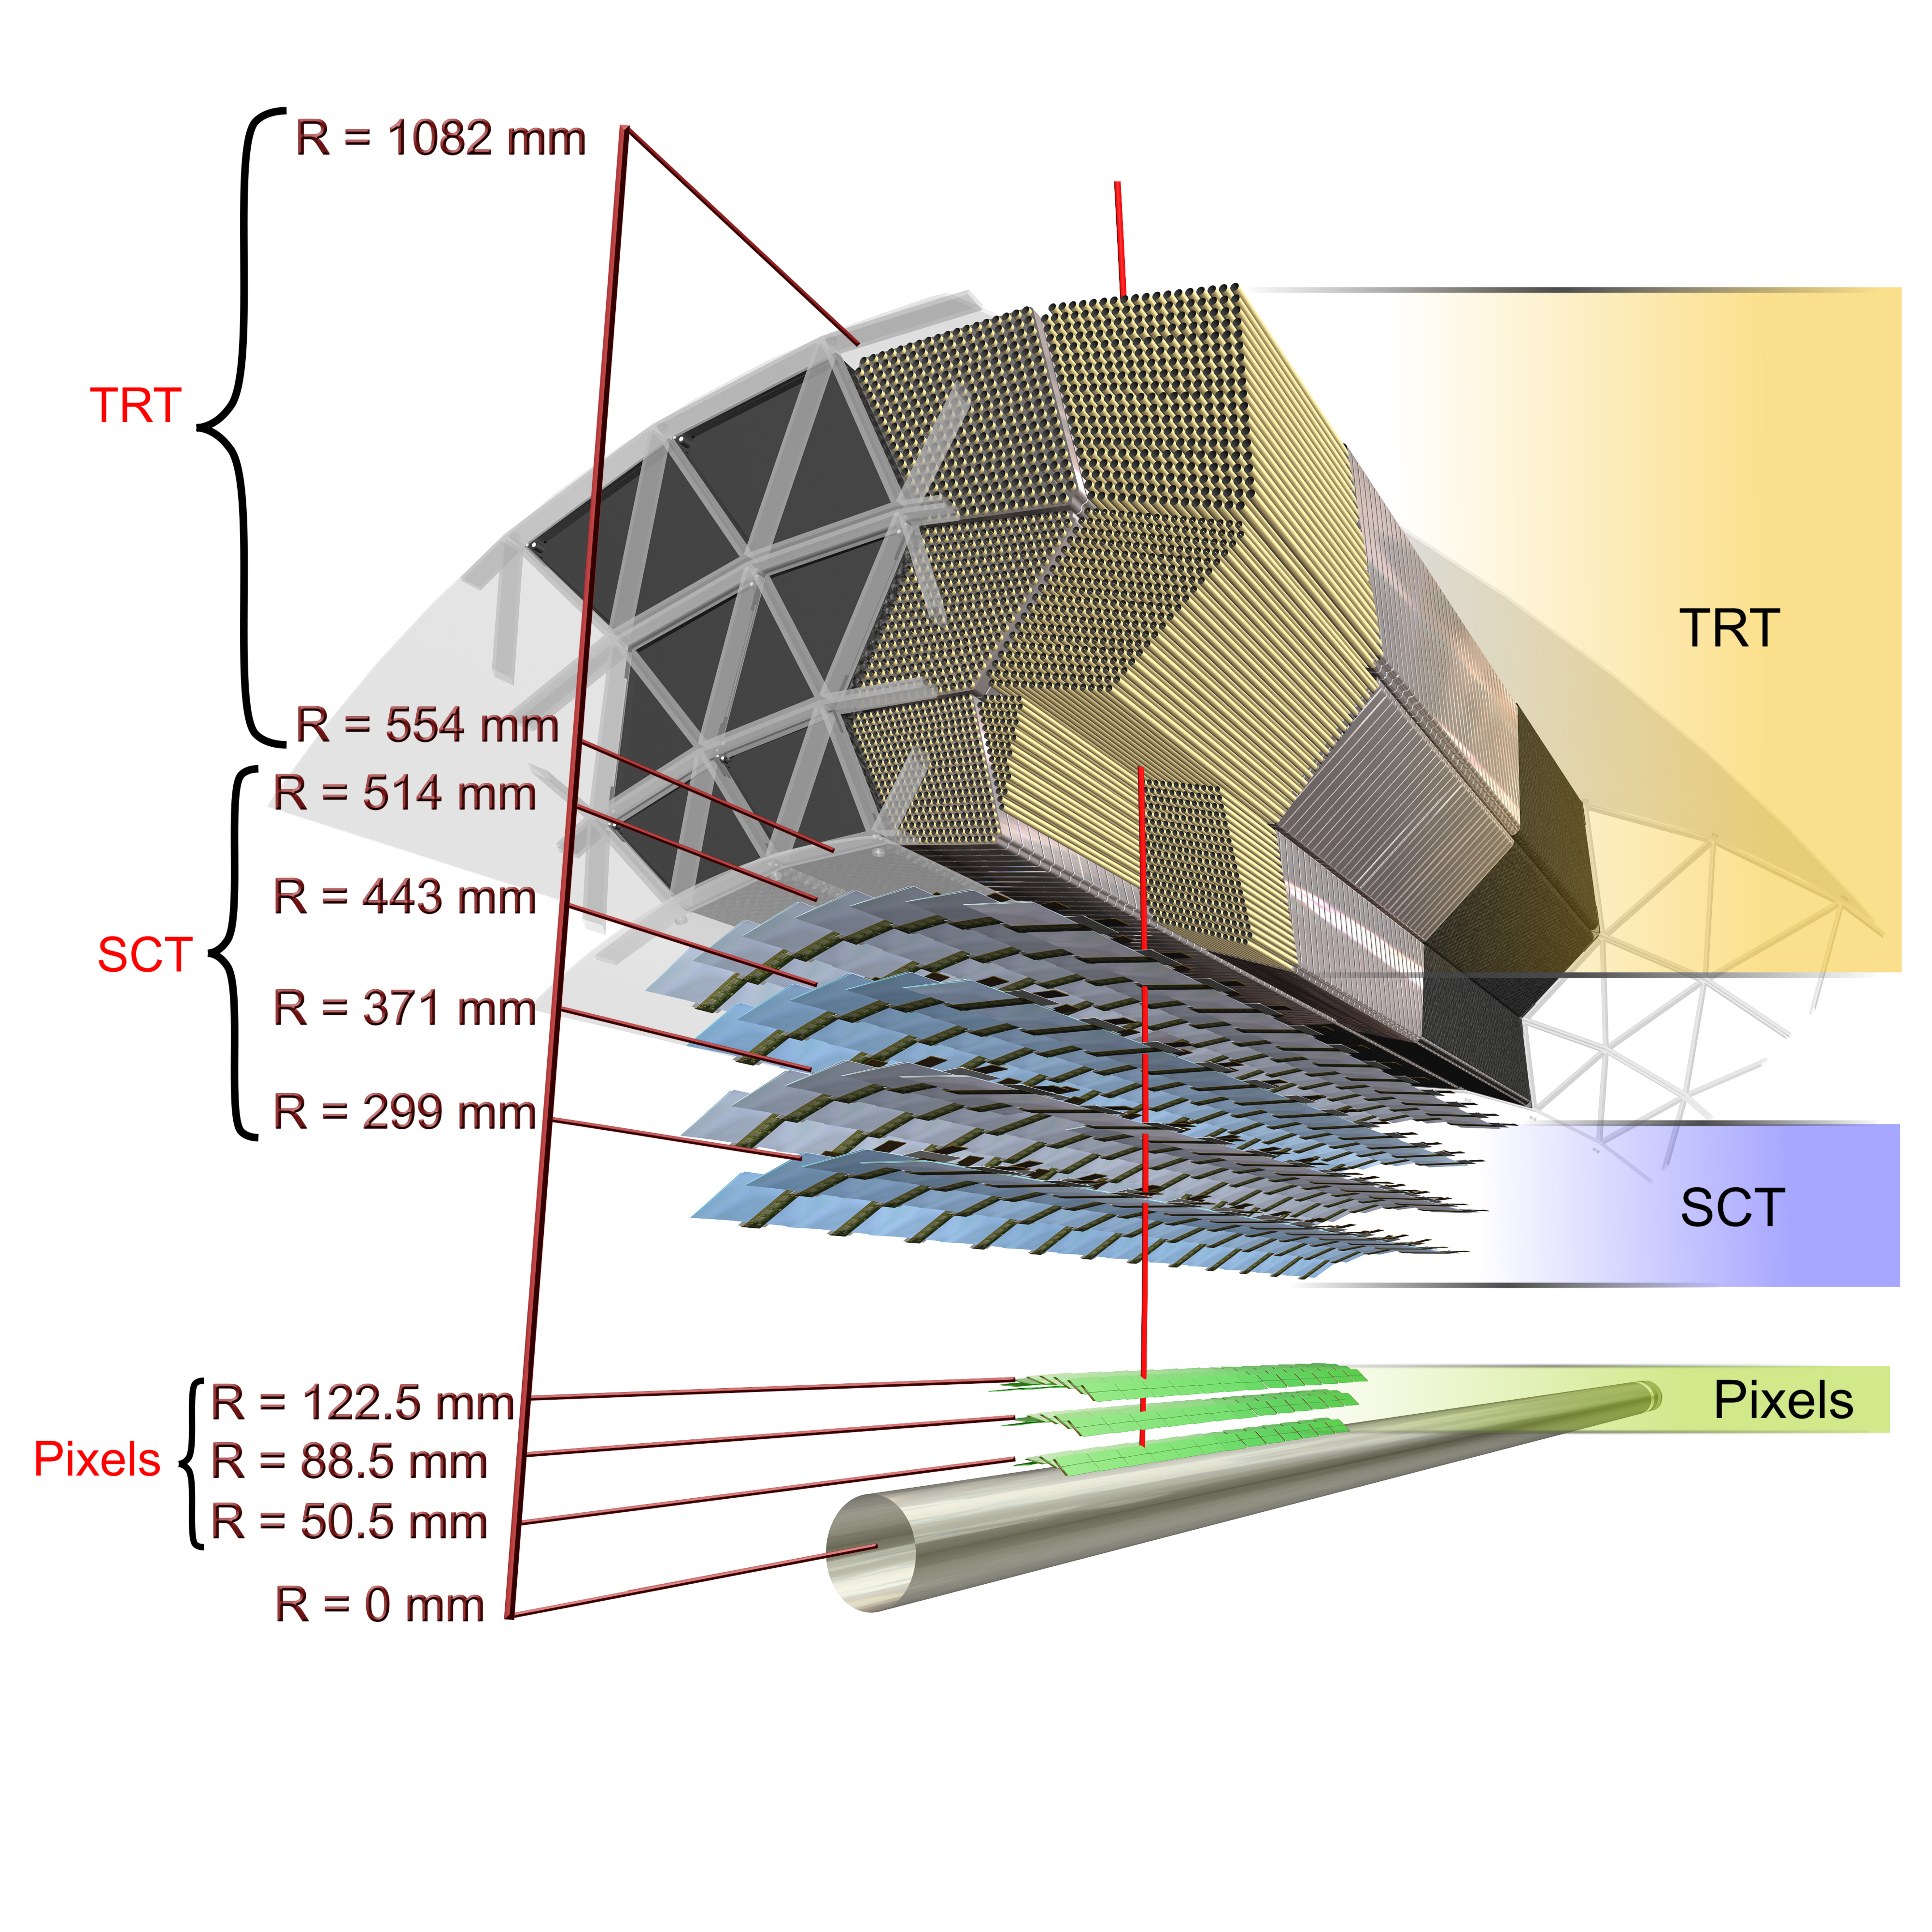
\includegraphics[width=0.8\textwidth]{fig/detector/inner_detector.pdf}
    \caption[]{}
\label{chap:detector:fig:inner_detector}
\end{figure}

\subsection{Silicon Detectors}

With nearly 50 $pp$ collisions per beam crossing producing $O(1000)$
particles per second, the detectors near the collision point are
required to have high resolution, fine granularity, fast response, and
radiation hardness. These requirements are satisfied by the silicon
pixel detectors. The 1744 identical pixel sensors of the pixel tracker
are arranged in three concentric layers in the barrel region
(figure~\ref{chap:detector:fig:inner_detector}) and in three disks in
each end-cap. Each sensor is composed of \textapprox{47k} pixels of
size $50~\mu\textrm{m} \times 400~\mu\textrm{m}$, corresponding to 80M readout
channels. The intrinsic spatial resolution of each pixel is
$10~\mu\textrm{m} \times 115~\mu\textrm{m}$, and the sensor is placed
such
that the precision pixel direction is the global azimuthal direction
in which charged particles bend. Due to the high efficiency of the
pixel sensors, the average charged particle
track in the ID volume will result in three precision spatial
measurements from the pixel tracker. 

Beyond the pixel detector lies the second silicon sub-detector in the
ID, the SCT. Due to budgetary constraints, the SCT relies on more
traditional technologies at the cost of degraded detector precision. In the
barrel region, the SCT modules are tiled to form four concentric
layers (figure~\ref{chap:detector:fig:inner_detector}), while in each
end-cap, the modules form nine disks, amounting to a total of 4088
modules. Each barrel module is composed of four nearly square
(64.0~mm~$\times$~63.6~mm) silicon
sensors, each with 768 readout strips that are $22~\mu\textrm{m}$ in
width~\cite{bib:Abdesselam:2006wt}. Two sensors are placed
side-to-side--- with a 2 mm gap for readout electronics--- on top of a
thermal pyrolitic graphite substrate, which provides mechanical
support and the thermal conductivity necessary for cooling the
sensors. Another two sensors are placed on the other side of the
substrate, and displaced by an angle of 40 mrad. This stereo angle
configuration allows another spatial degree of freedom to be
measured ($z$ in barrel, $R$ in endcap). The end-cap sensors and
modules are similar except for adjustments to the dimensions. The
intrinsic resolution of the SCT is $17~\mu\textrm{m}$ in
the azimuthal direction, and the effective resolution in the $z$ ($R$)
direction in the barrel (endcap) is $580~\mu\textrm{m}$. An average
track in the ID volume will result in four precision spatial
measurements in the SCT. 

\subsection{Transition Radiation Tracker}

The TRT is the outermost sub-detector in the ID, spanning the region
$56~\textrm{cm} < R < 108~\textrm{cm}$ in the
barrel~\cite{bib:Abat:2008zzb}. It is a collection of polyimide-based
drift chamber tubes (straws) that are 4~mm in diameter. The tube wall is the high
voltage cathode composed of layers of polyimide, graphite-polyimide,
polyurethane, and a 0.2 \micron layer of aluminium to achieve the
requisite electrical and mechanical properties~\cite{bib:Aad:2008zzm}. The anode is a
31 \micron gold-plated tungsten wire running directly through the
center of the straw with a radial offset of less than
300 \micron. Each straw is filled with a gas mixture of 70\% Xe, 27\%
CO$_2$, and 3\% O$_2$. 

In the TRT barrel region, spanning $|\eta| < 1.0$, the TRT straws run
parallel to the beam axis. They are placed in carbon-fiber-shelled modules
in which the straws form uniform arrays with an average spacing of
6.6~mm. The straws in the module are 144~cm long. To accomodate high
particle multiplicity, the wires within each straw are electrically
disconnected at the straw center, allowing two independent measurements
from a single straw. At either end of the module, there is a high
voltage plate that couples to the straw walls and a front-end
electronics board. A gas inlet circulates CO$_2$ outside of the
straws, thereby preventing electrical discharges and the accumulation
of any leaked Xe. This gas bath also cools the straws by conducting
heat to the highly thermally-conductive shell of the module. With a
quadralateral prism geometry, the modules are
arranged into three concentric rings, each comprised of 32 modules. 

The TRT end-caps provide tracking in the region $1.0 < |\eta| <
2.0$. Each end-cap consists of two sets of wheels. The set closer to
the collision point is composed of 12 wheels, each with eight straw
layers spaced at a wire-to-wire distance of
8~mm~\cite{bib:Abat:2008zz}. The other wheel set
has only eight wheels and a layer spacing of 15~mm. In each wheel,
there are 768 straws of length 37~cm oriented radially outwards with
uniform azimuthal spacing. To achieve better uniformity in the number
of straws that are traversed, each successive wheel is rotated by
$3/8$ of the azimuthal spacing. Similar to the barrel modules, each
wheel is a self-contained unit in which CO$_2$ circulates around the
straws. 

In total, there are 52544 straws in the barrel and 122880 straws in each
end-cap. On average, a charged particle with a momentum greater than
$500 \mev$ and $|\eta| < 2.0$ will traverse 36 straws, except in the
transition region between the barrel and end-cap, $0.8 < |\eta| <
1.0$. Each straw is capable of providing a measurement of the distance
of closest approach in the plane perpindicular to the straw direction
at an intrinsic resolution of 130 \micron. Therefore, in the barrel
(end-cap), the TRT measures an $R-\phi$ ($z-\phi$) coordinate but no $z$
($R$) information. 

\note{I should probably include a paragraph on electron ID capability}
